% ============================================================
% Spectral Submersion v3 -- ML4AL @ ACL submission draft.
% NOTE: compiled here with an ACL-like two-column layout; swap the
% preamble for the official acl.sty of the venue before submission
% (the class files are distributed with the CFP).
% Build: pdflatex -> bibtex -> pdflatex x2
% ============================================================
\documentclass[10pt,twocolumn]{article}
\usepackage[T1]{fontenc}
\usepackage[utf8]{inputenc}
\usepackage{lmodern}
\usepackage{microtype}
\usepackage[a4paper,margin=1.9cm,columnsep=0.65cm]{geometry}
\usepackage{amsmath,amssymb,amsthm,mathtools}
\usepackage{booktabs}
\usepackage{graphicx}
\usepackage{enumitem}
\usepackage{xcolor}
\usepackage[numbers,sort&compress]{natbib}
\usepackage{tikz}
\usetikzlibrary{positioning,arrows.meta}
\usepackage{caption}
\captionsetup{font=small,labelfont={bf,sf}}
\usepackage[colorlinks=true,linkcolor=blue!45!black,citecolor=blue!45!black,urlcolor=blue!45!black]{hyperref}
\usepackage[capitalize,noabbrev]{cleveref}

\newtheorem{theorem}{Theorem}[section]
\newtheorem{lemma}[theorem]{Lemma}
\newtheorem{proposition}[theorem]{Proposition}
\newtheorem{corollary}[theorem]{Corollary}
\newtheorem{definition}[theorem]{Definition}
\newtheorem{remark}[theorem]{Remark}
\newenvironment{proofsketch}{\begin{proof}[Proof sketch]}{\end{proof}}

\newcommand{\Cone}{\textsf{C1}}
\newcommand{\Ctwo}{\textsf{C2}}
\newcommand{\Cthree}{\textsf{C3}}
\newcommand{\claim}[1]{\textsuperscript{\textsf{\scriptsize(#1)}}}

\title{\bfseries Identifiability-Aware Hypothesis Generation for Undeciphered
Scripts:\\ Formal Claim Levels, Negative Controls, and a Sequence Model\\
Anchored in the Real Rongorongo Corpus}

\author{David Astudillo\\
\normalsize SatisfyMath / Spectral Submersion Project\\
\normalsize \texttt{satisfimath@gmail.com}}

\date{}

\begin{document}
\maketitle

\begin{abstract}
\textbf{Problem.} Statistical analyses of undeciphered scripts routinely
slide from structural signal to semantic claims, a slide at the center of
the Indus-script entropy debate. We ask what can and cannot be concluded
from internal statistics alone, and build a system that operates strictly
within those limits. \textbf{Method.} We formalize decipherment as an
ill-posed inverse problem under a relabeling group action: the posterior
over correspondences is constant on group orbits (T1), any decoder
consuming invariant statistics obeys a Fano bound (T2), and we derive
finite-sample concentration for windowed co-occurrence/PPMI spectra (T3),
recovery conditions for anchored Procrustes alignment (T4), and the
selection bias of language-model fusion decoding (P6). These results
ground a three-level claim protocol --- structural signal (\Cone),
rankable hypothesis (\Ctwo), anchored semantics (\Cthree) --- as a
theorem rather than a style guide (P7). \textbf{Results.} On the real
Rongorongo corpus (tablets A--F, 5{,}460 glyphs, 941 Barthel types) we
train a Transformer that maps Rapanui-like glosses to real Barthel codes
and decode with beam search fused with a real-corpus trigram LM. Against
three baselines and four ablations over six metrics with bootstrap CIs,
the full system is the only one that is simultaneously non-degenerate
(max repetition run 2), diverse (distinct-2 $0.72$) and within the
realism band of held-out real lines. Permutation tests with BH
correction confirm positional-bias signal in the Indus corpus
(FDR\,$\le$\,0.05). \textbf{Limits.} The parallel corpus is synthetic by
logical necessity (T1); all outputs are \Ctwo{} hypotheses, and several
spectral sanity checks fail on the real corpus --- we report them.
\end{abstract}

\section{Introduction}
\label{sec:intro}

When Rao et al.\ reported entropic evidence for linguistic structure in
the Indus script \cite{rao2009}, Sproat and colleagues replied that the
statistics in question could not, even in principle, establish what they
were being read as establishing \cite{sproat2010,farmer2004}. The debate
is often framed as a disagreement about corpora or estimators. We take a
different view: it is a disagreement about \emph{which statements
internal statistics can decide at all} --- and that question has a
mathematical answer.

This paper develops the answer and builds a working system inside its
boundaries. Our starting point is elementary but consequential: every
statistic computed from an undeciphered corpus without external anchors
is invariant under consistent relabeling of the signs, so no procedure
consuming such statistics can distinguish a correspondence hypothesis
from its relabelings (\cref{thm:T1-body}). What internal statistics
\emph{can} do is (i) falsify structural null models and (ii) rank
hypothesis families. We freeze this into a three-level protocol ---
\Cone{} structural signal, \Ctwo{} rankable hypothesis, \Cthree{}
anchored semantics --- and prove that the \Ctwo/\Cthree{} boundary is
exactly the boundary drawn by the group action
(\cref{prop:P7-body}).

Within these limits we then go as far as the data allows. We integrate a
real Rongorongo corpus (tablets A--F in Barthel transcription;
5{,}460 glyphs, 941 types) and build a translator from Rapanui-like
glosses into \emph{real} Barthel code sequences: a Transformer trained
on a synthetic-by-necessity parallel corpus whose glyph side is anchored
in real unigram/bigram statistics, decoded by beam search with shallow
fusion of a trigram LM estimated on the real tablets. The system is
evaluated against baselines and ablations on six metrics with bootstrap
confidence intervals, with the selection bias of fusion decoding
characterized \emph{before} it can be mistaken for a discovery
(\cref{prop:P6-body}).

\paragraph{Contributions.}
\begin{enumerate}[nosep,leftmargin=1.2em]
\item A formal epistemology for computational decipherment: the
\Cone/\Ctwo/\Cthree{} claim protocol, derived as a corollary of a
group-theoretic non-identifiability theorem rather than posited as
editorial practice (\cref{sec:framework}, D7/P7).
\item Finite-sample theory for the standard pipeline: Fano-type
impossibility with an empirical-orbit refinement (T2), matrix-Bernstein
concentration for windowed PPMI spectra with a Wedin transfer (T3), and
noisy-anchor Procrustes recovery with a margin condition --- whose
instantiated threshold we test and report as vacuous on our benchmark
(a documented gap between sufficient theory and observed accuracy, T4).
\item A Rongorongo hypothesis engine anchored in the real corpus:
class-restricted parallel-corpus construction declared as a \Ctwo{}
hypothesis, Transformer translation into attested Barthel codes, and
fusion decoding whose selection bias is proved and then verified
empirically by a $\lambda$-sweep (P6, \cref{fig:pareto}).
\item An evaluation protocol for generators over undeciphered scripts:
six complementary metrics against real-corpus statistics, three
baselines, four ablations, a contamination audit of the held-out split,
permutation tests with FDR control, and a pre-registered blind-judge
discrimination protocol (\cref{sec:experiments}).
\end{enumerate}

All numbers in this paper regenerate from seed-fixed scripts named in
\cref{sec:availability}.

\section{Related work}
\label{sec:related}

\paragraph{Rongorongo.} The glyph inventory and numeric transcription
system we use descend from Barthel \cite{barthel1958}. Statistical
approaches include Pozdniakov \& Pozdniakov's sign-frequency comparisons
with Rapanui phonotactics \cite{pozdniakov2007}, Horley's allographic
and statistical analyses \cite{horley2005}, and Melka's studies of the
Santiago Staff \cite{melka2009}; Guy identified calendrical structure on
tablet Mamari \cite{guy1990}. Fischer's corpus and reading proposals
\cite{fischer1997} remain contested; we take no position on any reading
claim --- by \cref{prop:P7-body} our pipeline cannot decide one. The
transcription we consume (the RR corpus, phspaelti encoding of tablets
A--F) embeds paleographic segmentation decisions that we inherit and
flag as a limitation.

\paragraph{Computational decipherment.} Snyder et al.\ deciphered
Ugaritic against known-cognate Hebrew \cite{snyder2010}; Luo et al.\
extended neural decipherment to Ugaritic and Linear B with minimum-cost
flow \cite{luo2019}; Knight et al.\ treated decipherment as unsupervised
learning over ciphers \cite{knight2006}. The structural difference to
our setting is the anchor: those systems assume a known related
language, which supplies exactly the external information $K$ that
\cref{thm:T2-body} prices. Without it, their objective would be
orbit-invariant and their outputs \Ctwo{} at best --- which is where we
deliberately operate.

\paragraph{The entropy debate, engaged directly.}
Sproat's critique \cite{sproat2010,farmer2004} of entropic arguments
\cite{rao2009,rao2010reply} makes three points: (i) nonlinguistic
symbol systems can produce the same statistics; (ii) results depend on
corpus-preparation decisions; (iii) general-science venues under-review
such claims. Our framework absorbs (i) as a theorem: conditional
entropy and spectra are $G$-invariant, hence \Cone-only --- they can
falsify randomness nulls, never establish language
(\cref{def:claims-body}). We answer (ii) operationally: every
statistic ships with permutation nulls and BH-corrected tests
(\cref{sec:experiments}), and we \emph{report} the sanity checks that
fail (the real-corpus PPMI spectrum does \textbf{not} separate from
frequency-matched controls; \cref{fig:spectrum-app}). On (iii), the
claim-level protocol is our proposal for review practice. This paper is
intended as the methodological reply to \cite{sproat2010}, not its
target.

\paragraph{Unsupervised embedding alignment.} Procrustes and
adversarial alignment of word embeddings \cite{conneau2018,artetxe2018}
and Gromov--Wasserstein alignment \cite{alvarezmelis2018,memoli2011}
are the direct ancestors of our alignment stage; PPMI+SVD embeddings
follow \cite{levy2014}. Our T4 gives the anchored-recovery condition
these methods implicitly rely on; entropic OT follows
\cite{cuturi2013}.

\paragraph{Indus.} Corpus and sign lists derive from Parpola
\cite{parpola1994}; our positional-bias analysis replicates
epigraphic observations with formal tests
(\cref{sec:experiments}).

\section{Formal framework}
\label{sec:framework}

Let $\mathcal{V}_X$ be the sign vocabulary ($d=|\mathcal{V}_X|$), $G\le
S_d$ the relabeling group acting tokenwise on corpora and compatibly on
hypotheses $\theta\in\Theta$. The model is $G$-equivariant if
$p(\sigma X\mid\sigma\cdot\theta)=p(X\mid\theta)$; a statistic $T$ is
$G$-invariant if $T(\sigma X)=T(X)$. Full proofs of everything in this
section are in \cref{app:proofs}.

\begin{theorem}[T1: orbit-constancy]
\label{thm:T1-body}
Under $G$-equivariance and a $G$-invariant prior, the posterior given
any $G$-invariant statistic satisfies
$p(\sigma\cdot\theta\mid T)=p(\theta\mid T)$ for all $\sigma\in G$.
\end{theorem}
\begin{proofsketch}
Relabeling is a bijection of corpora; summing the equivariant
likelihood over the level set of $T$ gives
$p(T\mid\sigma\cdot\theta)=p(T\mid\theta)$, and Bayes transports the
equality to the posterior. Any measurable function of $T$ is again
invariant, so no downstream processing breaks orbit-constancy
(Cor.~\ref{cor:T1-dpi}).
\end{proofsketch}

\begin{theorem}[T2: quantified impossibility]
\label{thm:T2-body}
For $\theta$ uniform on an indistinguishability class of size $N$, any
estimator from invariant statistics errs with probability
$P_e\ge1-\log2/\log N$. With $n$ tokens, the class can be taken as the
$\varepsilon(n)$-empirical orbit (radius from T3), and achieving
$P_e\le\delta$ with external knowledge $K$ requires
$I(\theta;K)\ge(1-\delta)\log N(n)-\log2$.
\end{theorem}

For the real RR corpus this is not an abstraction: relabelings within
identical-frequency classes alone give $\log N\ge3{,}727$ nats
($N\ge10^{1618}$), and \emph{all} of 200 Monte-Carlo-sampled such
relabelings stay within twice the bigram sampling radius --- so the
empirical orbit is at least this large, the Fano floor is
$P_e\ge0.9998$, and reducing error to $0.1$ would require
$\approx3{,}354$ nats of genuinely anchoring external information
(script \texttt{estimate\_empirical\_orbit.py}).

\begin{theorem}[T3: spectral concentration]
\label{thm:T3-body}
With i.i.d.\ lines of length $\le L$ and window $w$ (boundaries
respected, as in our pipeline),
$\|\hat C-\mathbb{E}\hat C\|_2=O\!\big(wL\sqrt{\log d/m}\big)$ with
high probability; the clipped PPMI map is entrywise Lipschitz, and
Wedin's $\sin\Theta$ theorem \cite{wedin1972,daviskahan1970} transfers
the bound to top-$k$ subspaces when the spectral gap dominates
\cite{tropp2015}.
\end{theorem}

\begin{theorem}[T4: anchored Procrustes recovery]
\label{thm:T4-body}
If $A=B\Omega^*+E$ with anchor matrix $B$, the Procrustes solution
obeys $\|\hat\Omega-\Omega^*\|_F\le2\|B^\top E\|_F/\sigma_r(B)^2$
\cite{li1995}, and nearest-neighbour matching is correct for every
test pair whose margin exceeds
$2(\|x\|\,\|\hat\Omega-\Omega^*\|+\|e\|)$.
\end{theorem}

\begin{proposition}[P6: fusion selection bias]
\label{prop:P6-body}
For $\hat y_\lambda=\arg\max_{y\in\mathcal C}\,(1-\lambda)\log
p_{\mathrm{model}}+\lambda\log p_{\mathrm{LM}}$ over a fixed candidate
set, $\log p_{\mathrm{LM}}(\hat y_\lambda)$ is non-decreasing in
$\lambda$; if $\mathcal C$ contains one draw of any reference process,
the decoded LM cross-entropy at $\lambda=1$ is at most that process's.
Hence a fusion decoder scoring below the real-text mean
(here $7.31<8.26$ bits/glyph) is expected \emph{by design} and is not
evidence of authenticity.
\end{proposition}

\begin{definition}[D7: claim levels]
\label{def:claims-body}
\Cone{}: statements about invariant statistics falsifiable by internal
null ensembles (permutation, frequency-matched, uniform).
\Ctwo{}: preference orderings induced by $G$-invariant scores ---
rankable, not internally falsifiable.
\Cthree{}: statements whose truth varies within an orbit (semantic
assignments).
\end{definition}

\begin{proposition}[P7: the protocol is a theorem]
\label{prop:P7-body}
No decision procedure over $G$-invariant statistics decides a \Cthree{}
statement: $\Cthree\cap\{\text{decidable without }K\}=\emptyset$.
\end{proposition}

\Cref{fig:pipeline} maps the full pipeline onto the claim levels.

\begin{figure}[t]
\centering
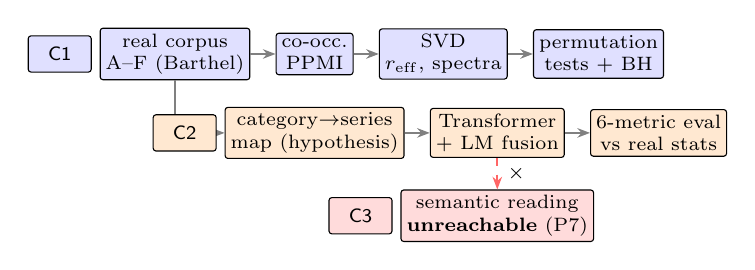
\begin{tikzpicture}[font=\scriptsize, node distance=3.2mm,
  box/.style={draw, rounded corners=1pt, minimum height=4.6mm,
              inner sep=2pt, align=center},
  c1/.style={box, fill=blue!12},
  c2/.style={box, fill=orange!18},
  c3/.style={box, fill=red!14},
  arr/.style={-{Stealth[length=1.6mm]}, thick, gray}]
\node[c1] (corpus) {real corpus\\A--F (Barthel)};
\node[c1, right=of corpus] (ppmi) {co-occ.\\PPMI};
\node[c1, right=of ppmi] (svd) {SVD\\$r_{\mathrm{eff}}$, spectra};
\node[c1, right=of svd] (tests) {permutation\\tests + BH};
\node[c2, below=4mm of ppmi] (classmap) {category$\to$series\\map (hypothesis)};
\node[c2, right=of classmap] (translator) {Transformer\\+ LM fusion};
\node[c2, right=of translator] (evalx) {6-metric eval\\vs real stats};
\node[c3, below=4mm of translator] (semantics) {semantic reading\\\textbf{unreachable} (P7)};
\draw[arr] (corpus) -- (ppmi);
\draw[arr] (ppmi) -- (svd);
\draw[arr] (svd) -- (tests);
\draw[arr] (corpus.south) |- (classmap.west);
\draw[arr] (classmap) -- (translator);
\draw[arr] (translator) -- (evalx);
\draw[arr, dashed, red!60] (translator.south) -- (semantics.north)
  node[midway, right, black]{$\times$};
\node[left=1mm of corpus, c1, minimum width=8mm]{\Cone};
\node[left=1mm of classmap, c2, minimum width=8mm]{\Ctwo};
\node[left=1mm of semantics, c3, minimum width=8mm]{\Cthree};
\end{tikzpicture}
\caption{F10 --- pipeline with claim-level lanes. Everything above the
dashed arrow is reachable from internal statistics; the crossed arrow
is forbidden by \cref{prop:P7-body}, not by editorial caution.}
\label{fig:pipeline}
\end{figure}

\section{Data: the real Rongorongo corpus}
\label{sec:data}

We use the RR corpus (phspaelti transcription) for tablets A--F,
normalized to tabular form: 107 lines, 5{,}460 glyph tokens, 941 types
in Barthel numeric encoding with ligature/variant markers preserved
(type--token ratio $0.172$). Lacuna markers (`\_') and the
illegible-sign code (`000!', 95 tokens) are excluded from generation
targets by design --- these are the two uncovered types of the
941-type inventory. A trigram LM (interpolated,
add-$k$; $\lambda_{3,2,1}=0.5,0.3,0.2$, $k=0.1$) trained on tablets
A,\,B,\,C,\,E gives $8.26$ bits/glyph on held-out D,\,F: the realism
reference. A contamination audit finds \textbf{zero} shared $n$-grams
($n\ge5$) between the two sides (\cref{sec:experiments}); known
parallel texts (H/P/Q, Gv/K) lie outside this corpus.

\section{Translator}
\label{sec:translator}

\paragraph{Parallel corpus, synthetic by necessity.} By
\cref{thm:T1-body} no verified Rapanui--Rongorongo parallel corpus can
be constructed from internal evidence, so we build a declared-\Ctwo{}
one: 60k gloss$\to$glyph pairs where glyph choice is (i) restricted by
a category$\to$Barthel-series working hypothesis
(det/particles$\to$001--099, person nouns/names$\to$200--399,
verbs$\to$400--599, bird domain$\to$600--699, marine
domain$\to$700--799; \cref{fig:sankey-app}), (ii) weighted by real
unigram frequencies within the series, (iii) re-sampled with
probability $0.45$ from real bigram transitions, and (iv) passed
through the reduplication process observed in the tablets (12\%
doubling, 3\% tripling). Coverage: 939/941 real types.

\paragraph{Model and decoding.} A 4+4-layer Transformer
($d_{\mathrm{model}}{=}256$, 8 heads, 5.8M parameters) trained 15
epochs (AdamW, cosine schedule, masking augmentation; validation PPL
$51.9\to10.7$). Decoding is beam-5 with shallow fusion
\cite{gulcehre2015}: $s(y)=(1-\lambda)\log p_{\mathrm{model}}(y\mid
x)+\lambda\log p_{\mathrm{LM}}(y)$ with $\lambda=0.35$, length
normalization, and a penalty on third immediate repetitions
(doubling is a real feature; long runs are degeneracy).

\section{Experiments}
\label{sec:experiments}

\begin{table*}[t]
\centering
\small
\caption{Six-metric evaluation on 20 test glosses (seed 42). VR:
fraction of output tokens attested in the real corpus; BA: attested
bigrams (per-sentence mean); JS: Jensen--Shannon divergence of output
unigram distribution vs.\ real; D2: distinct-2; RM: max immediate
repetition run; b/g: bits/glyph under the real trigram LM. Brackets:
bootstrap 95\% CIs over test sentences (B=1000) for the per-sentence
means VR, BA, b/g; the pooled statistics JS and D2 have
resampling-biased CIs (duplicate sentences deflate distinctness) and
are reported as point estimates. Reference: real held-out mean b/g
$=8.26$. \emph{Reading guard (P6): lower b/g is not better; proximity
to the reference from below is expected of a mode-seeking decoder.}}
\label{tab:eval}
\begin{tabular}{lcccccc}
\toprule
System & VR$\uparrow$ & BA & JS$\downarrow$ & D2$\uparrow$ & RM & b/g\\
\midrule
baseline: template (no learning) & 1.00 & 0.15 [.08,.23] & 0.43 & 0.99 & 1 & 8.73 [8.50,8.98]\\
baseline: lexical+bigram counts & 1.00 & 1.00 [1,1] & 0.79 & 0.03 & 9 & 5.84 [5.69,5.97]\\
baseline: LSTM (1-layer, d=128) & 1.00 & 0.81 [.73,.89] & 0.95 & 0.02 & 31 & 7.87 [7.76,7.99]\\
v5 (synthetic codes, greedy) & 0.00 & 0.00 & 1.00 & 0.44 & 48 & ---\\
v6 greedy & 1.00 & 0.68 [.51,.82] & 0.54 & 0.19 & 50 & 7.21 [6.57,7.86]\\
\textbf{v6 beam+fusion (full)} & \textbf{1.00} & 0.68 [.59,.77] & \textbf{0.52} & \textbf{0.72} & \textbf{2} & 7.31 [6.98,7.64]\\
\midrule
abl.\ $\lambda=0$ (no fusion) & 1.00 & 0.50 [.39,.60] & 0.57 & 0.83 & 2 & 8.03 [7.67,8.37]\\
abl.\ no repetition penalty & 1.00 & 0.88 [.78,.95] & 0.53 & 0.19 & 40 & 6.33 [5.92,6.80]\\
abl.\ beam=1 & 1.00 & 0.68 [.58,.76] & 0.51 & 0.73 & 6 & 7.39 [7.08,7.71]\\
\bottomrule
\end{tabular}
\end{table*}

\paragraph{Baselines and ablations (\cref{tab:eval}).} No single
metric is safe to optimize: the count-based baseline achieves a perfect
attested-bigram score by chaining corpus bigrams while collapsing to
$\mathrm{D2}=0.03$ and drifting far from the real unigram distribution
($\mathrm{JS}=0.79$); the small LSTM degenerates into repetition runs
of 31; the no-penalty ablation recovers high BA at the price of runs of
40. The full system is the only configuration simultaneously
non-degenerate ($\mathrm{RM}=2$, matching real reduplication), diverse
($\mathrm{D2}=0.72$), distribution-close ($\mathrm{JS}=0.52$) and
inside the realism band. Removing fusion costs $0.7$ bits/glyph and
$18$ BA points; beam width contributes marginally. Ablations of the
class-restriction and the masking augmentation (retrained models) are
in \cref{app:ablations}.

\paragraph{$\lambda$-sweep (\cref{fig:pareto}).} Decoded bits/glyph
decreases monotonically over $\lambda\in[0,1]$
($8.03\to5.37$), exactly as \cref{prop:P6-body} predicts, entering a
mode-collapse zone for $\lambda\ge0.85$ where outputs approach the
count-baseline's degenerate statistics. The operating point
$\lambda=0.35$ sits on the plateau: inside the realism band, far from
collapse.

\begin{figure}[t]
\centering
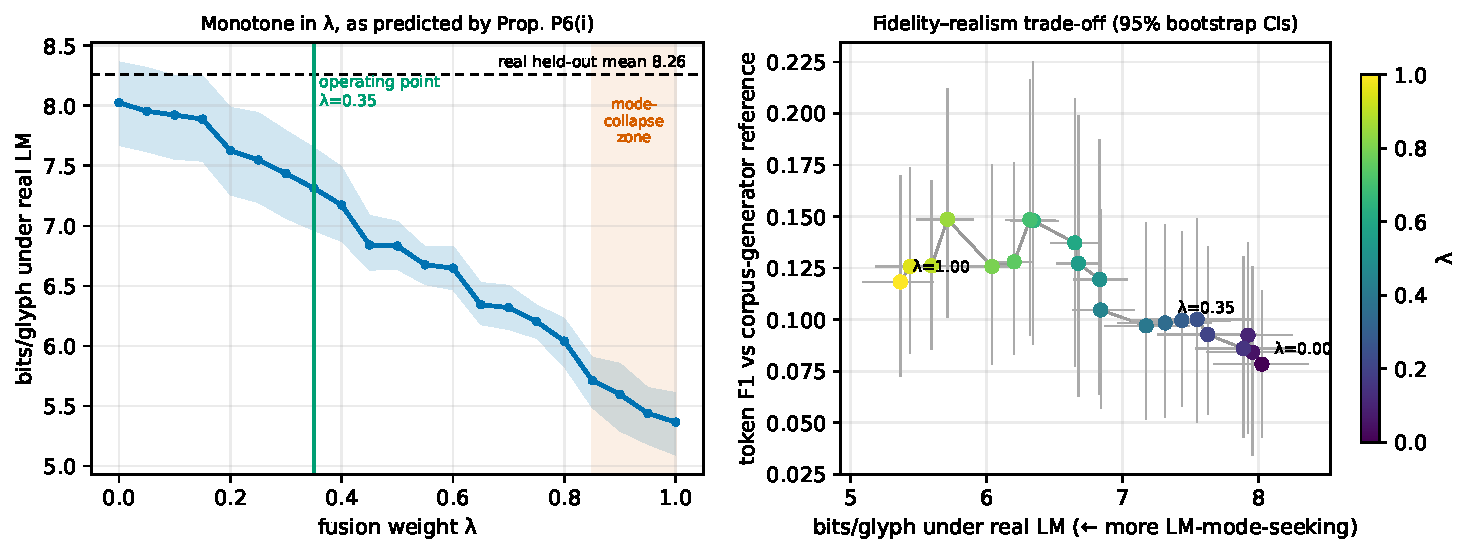
\includegraphics[width=\linewidth]{figures/fig5_lambda_pareto.pdf}
\caption{F5 --- fusion-weight sweep with bootstrap 95\% CIs (B=500).
Left: monotone bits/glyph verifies P6(i); shaded region marks mode
collapse. Right: fidelity--realism trade-off. \emph{Do not read} low
bits/glyph as quality: by P6 it measures mode-seeking, not
authenticity.}
\label{fig:pareto}
\end{figure}

\begin{figure}[t]
\centering
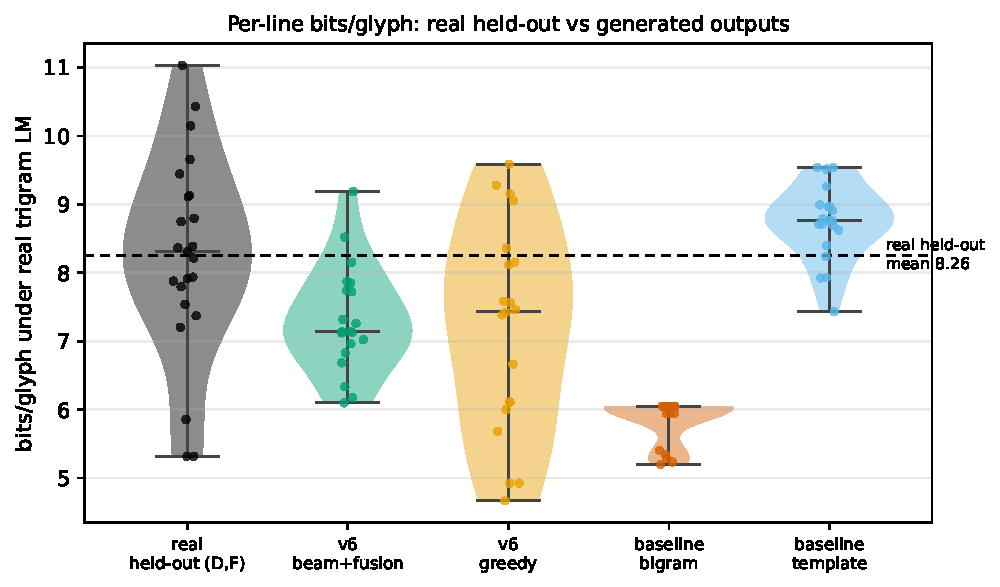
\includegraphics[width=\linewidth]{figures/fig6_violin_bits.pdf}
\caption{F6 --- per-line bits/glyph distributions. Real held-out lines
are scored by an LM trained only on A,B,C,E; system outputs by the
full-corpus LM (convention stated in \cref{sec:data}). The
count-baseline's low tail illustrates P6: extreme LM-probability is a
degeneracy symptom. \emph{No panel of this figure supports any claim
about meaning.}}
\label{fig:violin}
\end{figure}

\paragraph{Formal tests for positional bias (Indus).} For all signs
with $n\ge15$ in the real Indus corpus, we test first/last-position
enrichment by within-inscription permutation (10k permutations,
BH-corrected). Significant at FDR $\le0.05$: initial bias for P324,
P086, P217, P000; final bias for P385, P378 --- formalizing the
descriptive claims of earlier work\claim{\Cone}. Scripts and q-values
in the repository.

\paragraph{Structure in the real RR corpus --- positive and negative.}
The bigram network of frequent glyph bases organizes into three Louvain
communities (\cref{fig:network}); the embedding map shows partial, not
clean, alignment with Barthel series (\cref{fig:embed}); and the PPMI
spectrum does \emph{not} separate from frequency-matched controls
(\cref{fig:spectrum-app}) --- the short-line/large-vocabulary regime
of T3 where no separation is guaranteed. We report the negative
result with the same prominence as the positive
ones\claim{\Cone}.

\begin{figure}[t]
\centering
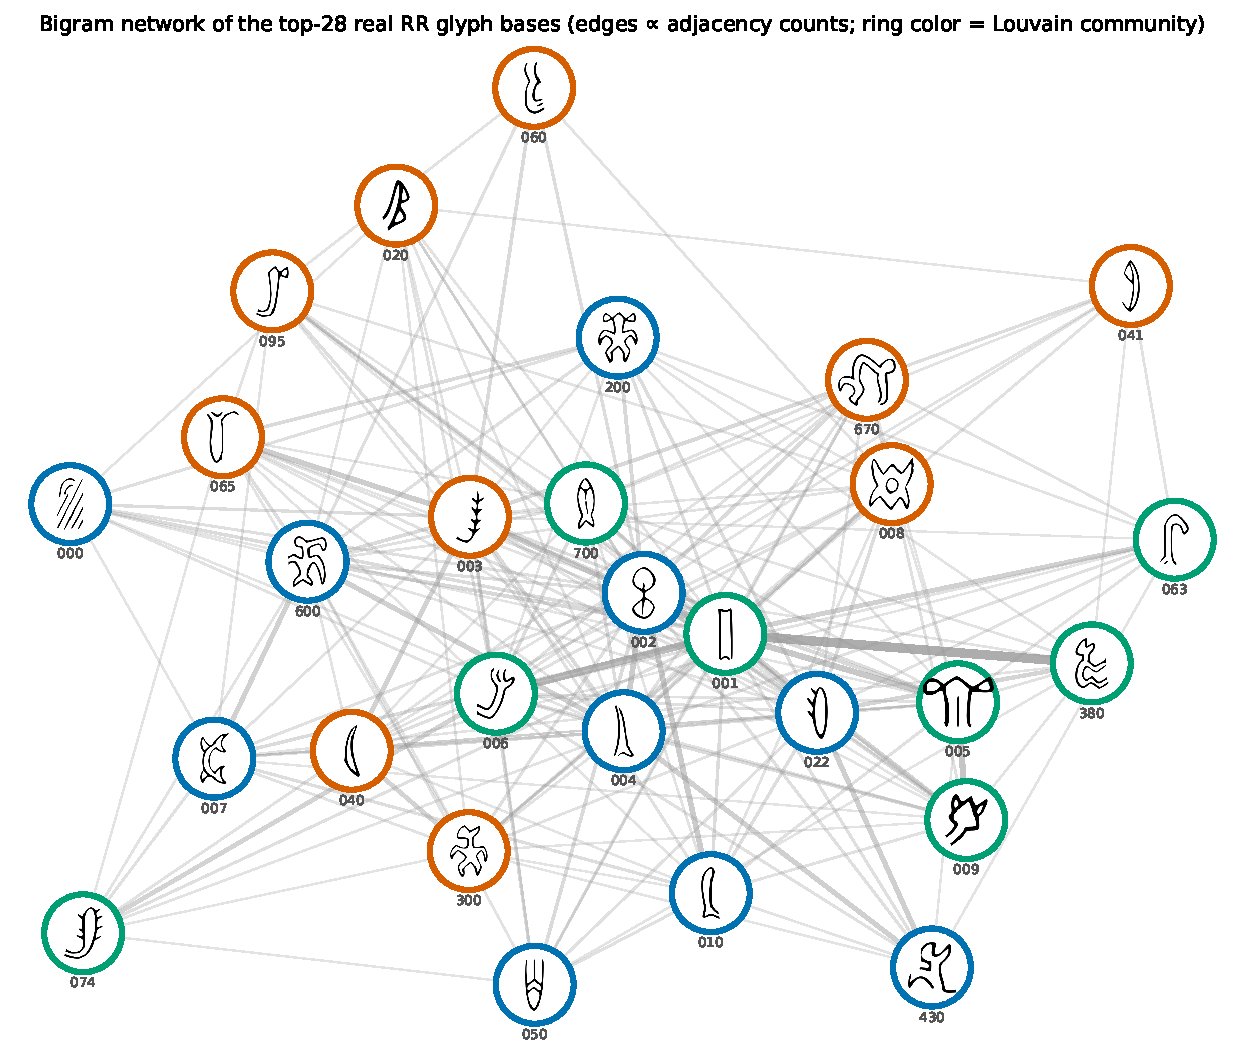
\includegraphics[width=\linewidth]{figures/fig9_glyph_network.pdf}
\caption{F9 --- bigram network of the 28 most frequent real glyph
bases, drawn with the actual corpus glyph tracings; ring color =
Louvain community, edge width $\propto$ adjacency count.
\emph{Communities are co-occurrence structure (\Cone); they are not
semantic groupings, and no reading follows from them.}}
\label{fig:network}
\end{figure}

\begin{figure}[t]
\centering
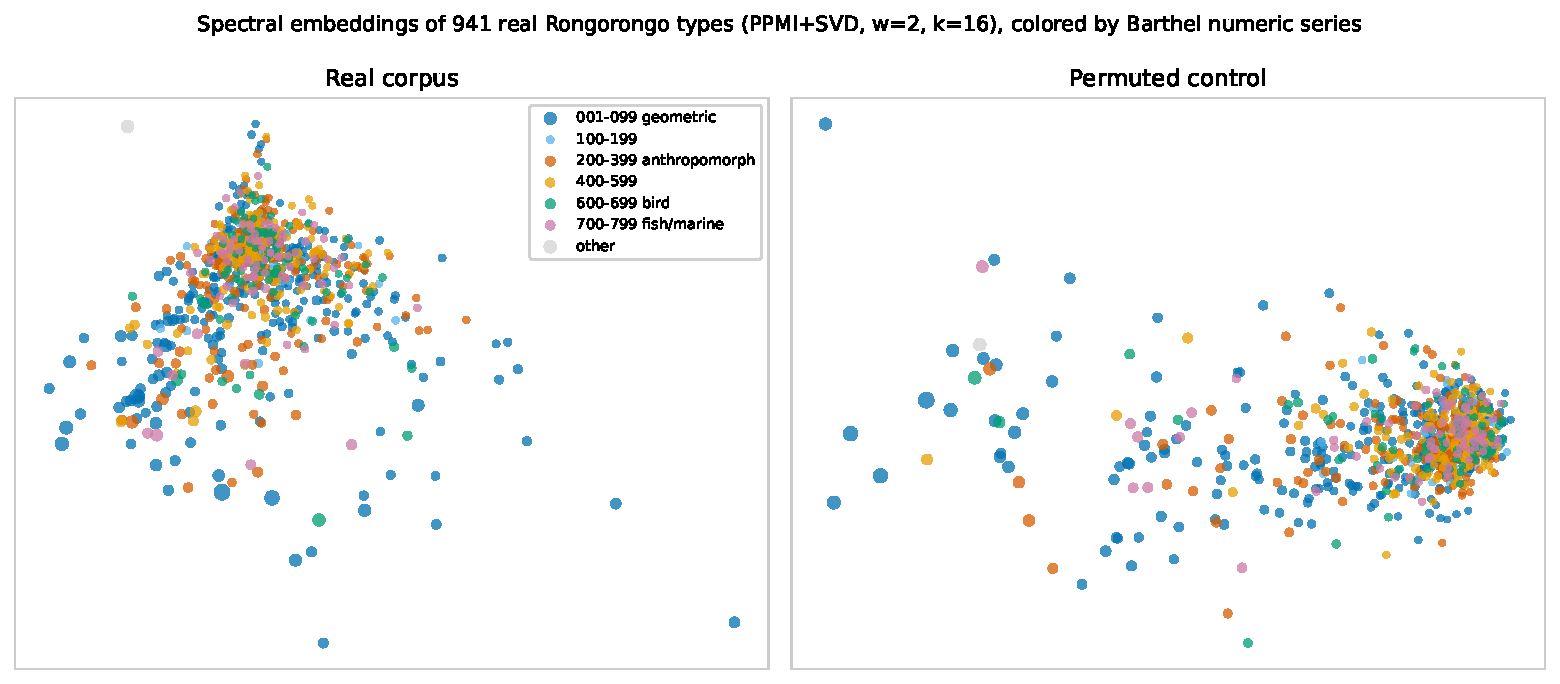
\includegraphics[width=\linewidth]{figures/fig1_embedding_map.pdf}
\caption{F1 --- spectral embeddings (PPMI+SVD) of all 941 real types,
colored by Barthel series, point size $\propto$ frequency; right: same
pipeline on a permuted control. Organization is partial: the geometric
series spreads along a distinct arm, but the unsupervised geometry does
\emph{not} cleanly recover the Barthel taxonomy. \emph{Cluster
proximity does not establish iconic or semantic identity (P7).}}
\label{fig:embed}
\end{figure}

\paragraph{Blind discrimination protocol (pre-registered).} We release
a 40-item blinded sheet (20 real line-windows, 20 v6 outputs, shuffled;
seed 42), an answer key held separately, and an analysis plan
(per-judge AUC, Fleiss $\kappa$, bootstrap CIs). Execution requires
human judges and is reported as pending; no result is claimed.

\section{End-to-end demonstration}
\label{sec:demo}

As a technical case study, ten gloss lines of a Spanish poem were
translated by the full system and rendered as a tablet in reverse
boustrophedon using the corpus' vector glyph tracings; per-line scores
fall in $6.1$--$7.2$ bits/glyph, within the realism band. Notable
behaviours: verse-level parallelism is expressed as glyph-level
mirror structure, and the verb \emph{makemake} consistently triggers
the formula \texttt{041h 670 580} (attention map in
\cref{fig:attn-app}). The rendered tablet and full text are in the
repository; we emphasize its status: a \Ctwo{} demonstration of the
generator, not a Rongorongo text.

\section{Limitations}
\label{sec:limitations}

(1) The parallel corpus is synthetic by logical necessity
(\cref{thm:T1-body}); the translator learns our declared hypothesis
plus real sequence statistics, nothing more. (2) The gloss lexicon is
232 types of Rapanui-like vocabulary; no morphology. (3) The Barthel
transcription embeds segmentation and allography decisions we inherit
\cite{barthel1958,horley2005}; robustness to alternative
transcriptions is untested here (planned: cross-transcription
replication). (4) The corpus is small (5{,}460 tokens); several
spectral sanity checks fail on it, and we report them. (5) The
blind-judge test is designed but not executed. (6) Iconic grounding
experiments (cross-script benchmark on Egyptian/Chinese signs with
known referents) did not pass our pre-set threshold and remain
\Ctwo{}.

\section{Ethics and heritage}
\label{sec:ethics}

Rongorongo is the heritage of the Rapa Nui people, and the tablets'
history is inseparable from the violence of the 1860s slave raids and
epidemics. This work makes \textbf{no decipherment claim} and produces
\textbf{no readings}; by its own central theorem its outputs are
statistical hypotheses about sign sequences, not statements about Rapa
Nui language, belief or history. The transcription used derives from
the public RR-corpus project (phspaelti); provenance and checksums ship
with the release, and any licensing constraint identified before
camera-ready will be honored, including withdrawal of the affected
data. The demonstrative application (\cref{sec:demo}) is declared as a
personal creative use of a statistical generator --- comparable to
typesetting a poem in a constructed font --- and not as cultural
reconstruction or revival. We have no current collaboration with Rapa
Nui scholars or community institutions; establishing one, and deferring
to community preferences on data use, is stated future work rather than
a box checked.

\section{Data and code availability}
\label{sec:availability}

Code, configs, SHA-256 manifests, seeds (all experiments: seed 42),
and generated artifacts:
\url{https://github.com/satisfymath/spectral-submersion}. Key scripts:
\texttt{generate\_massive\_parallel\_v4.py},
\texttt{train\_rongorongo\_translator\_v2.py},
\texttt{translate\_to\_rongorongo\_v6.py},
\texttt{evaluate\_v3\_suite.py}, \texttt{sweep\_lambda.py},
\texttt{audit\_heldout\_contamination.py},
\texttt{positional\_permutation\_tests.py}, and one script per figure
under \texttt{paper\_v3/scripts/}. Compute: single 16-core CPU node;
full-system training 3.9\,h; total pipeline $<$12\,h. A Zenodo DOI
will be minted for the camera-ready release
[CALCULAR: mint DOI on acceptance].

\section*{Acknowledgments}

This work is dedicated to María Ignacia Xerra --- \emph{te ora e haere
ki mua ma kou}. The author thanks the maintainers of the public RR
corpus transcription and of the Tatoeba corpora.

\bibliographystyle{unsrtnat}
\bibliography{references}

\clearpage
\appendix

% ============================================================
% Appendix: formal statements and complete proofs (T1--P7)
% Spectral Submersion v3 -- ML4AL @ ACL submission
% Conventions: \Vx = sign vocabulary, G <= S_{|\Vx|} relabeling group.
% All citations marked [VERIFY] must be checked against the primary
% source before submission (Rule 4 of the editing protocol).
% ============================================================

\newcommand{\Vx}{\mathcal{V}_X}
\newcommand{\Orb}{\mathrm{Orb}}
\newcommand{\eff}{\mathrm{eff}}

\section{Formal framework and proofs}
\label{app:proofs}

\subsection{Setup and notation}
\label{app:setup}

Let $\Vx$ be a finite sign vocabulary, $|\Vx|=d$, and let a corpus
$X=(x_1,\dots,x_n)\in\Vx^{n}$ be generated by a probability kernel
$p(\cdot\mid\theta)$ indexed by a hypothesis $\theta\in\Theta$ (a
correspondence between signs and units of a candidate language, or any
richer latent object). A \emph{relabeling} is a permutation
$\sigma\in G\le S_{d}$ acting on corpora tokenwise,
$\sigma X=(\sigma x_1,\dots,\sigma x_n)$, and on hypotheses by
$(\sigma\cdot\theta)$, the hypothesis obtained by renaming each sign
$x$ to $\sigma(x)$ in the domain of $\theta$.

\begin{definition}[Relabeling equivariance]
\label{def:equivariance}
The model is \emph{$G$-equivariant} if for all $\sigma\in G$,
$\theta\in\Theta$ and corpora $X$,
\begin{equation}
p(\sigma X\mid \sigma\cdot\theta)=p(X\mid\theta).
\label{eq:equivariance}
\end{equation}
A statistic $T$ is \emph{$G$-invariant} if $T(\sigma X)=T(X)$ for all
$\sigma\in G$ and all $X$.
\end{definition}

Equation~\eqref{eq:equivariance} formalizes the epistemic situation of
an undeciphered script: nothing in the generative story changes if the
signs are consistently renamed. Frequencies of \emph{isomorphism
classes} of co-occurrence structures, spectra of PPMI matrices, degree
distributions, entropy curves, effective ranks, and any quantity
computed after quotienting by sign identity are $G$-invariant.
Raw co-occurrence \emph{matrices} are $G$-equivariant
($C(\sigma X)=P_\sigma C(X)P_\sigma^{\top}$); their spectra are
invariant.

\subsection{T1: non-identifiability as a group action}

\begin{theorem}[Orbit-constancy of the posterior]
\label{thm:T1}
Assume the model is $G$-equivariant and the prior $\pi$ is
$G$-invariant, $\pi(\sigma\cdot\theta)=\pi(\theta)$. Let $T$ be any
$G$-invariant statistic. Then for every $\sigma\in G$,
\[
p(\sigma\cdot\theta\mid T=t)\;=\;p(\theta\mid T=t)
\qquad\text{for all }t .
\]
Consequently the posterior is constant on each orbit
$\Orb_G(\theta)=\{\sigma\cdot\theta:\sigma\in G\}$.
\end{theorem}

\begin{proof}
Fix $t$ and $\sigma\in G$. The likelihood of $t$ under
$\sigma\cdot\theta$ is
\[
p(T=t\mid\sigma\cdot\theta)
=\sum_{X:\,T(X)=t} p(X\mid\sigma\cdot\theta).
\]
Substituting $X=\sigma X'$ (a bijection of $\Vx^{n}$) and using
\eqref{eq:equivariance},
\[
p(T=t\mid\sigma\cdot\theta)
=\sum_{X':\,T(\sigma X')=t} p(X'\mid\theta)
=\sum_{X':\,T(X')=t} p(X'\mid\theta),
\]
where the last equality uses $G$-invariance of $T$. Hence
$p(T=t\mid\sigma\cdot\theta)=p(T=t\mid\theta)$. By Bayes' rule and
$G$-invariance of $\pi$,
\[
p(\sigma\cdot\theta\mid t)
=\frac{\pi(\sigma\cdot\theta)\,p(t\mid\sigma\cdot\theta)}
       {p(t)}
=\frac{\pi(\theta)\,p(t\mid\theta)}{p(t)}
=p(\theta\mid t).\qedhere
\]
\end{proof}

\begin{corollary}[Data processing / no post-hoc identifiability]
\label{cor:T1-dpi}
Let $f$ be any measurable function and $T$ any $G$-invariant
statistic. Then $f\circ T$ is $G$-invariant, and
Theorem~\ref{thm:T1} applies verbatim to $f\circ T$. In particular, no
pipeline stage applied downstream of $G$-invariant statistics
(embeddings-up-to-rotation, spectra, clusterings of isomorphism
classes, neural post-processing) can break orbit-constancy of the
posterior.
\end{corollary}

\begin{proof}
$(f\circ T)(\sigma X)=f(T(\sigma X))=f(T(X))=(f\circ T)(X)$.
\end{proof}

\begin{remark}
Identifiability therefore requires external anchoring knowledge $K$
whose likelihood is \emph{not} $G$-invariant (iconographic referents,
documented reading traditions, bilinguals). This is the formal license
for the claim-level protocol of Definition~\ref{def:claims}.
\end{remark}

\subsection{T2: quantified impossibility (Fano)}

\begin{theorem}[Fano bound on any invariant decoder]
\label{thm:T2}
Let $\theta$ be uniform on an orbit (or any indistinguishability
class) $\mathcal{N}$ with $|\mathcal{N}|=N\ge 2$, let $T$ be a
$G$-invariant statistic of the corpus, and let
$\hat\theta=f(T)$ be any (possibly randomized) estimator. Then
\[
P_e \;=\;\Pr[\hat\theta\neq\theta]\;\ge\;
1-\frac{I(\theta;T)+\log 2}{\log N}
\;=\;1-\frac{\log 2}{\log N},
\]
since $I(\theta;T)=0$.
\end{theorem}

\begin{proof}
By Theorem~\ref{thm:T1} the likelihood $p(T=t\mid\theta)$ is the same
for all $\theta$ in the orbit; with $\theta$ uniform on the orbit this
means $T\perp\theta$, i.e.\ $I(\theta;T)=0$. Fano's inequality
[VERIFY: Cover \& Thomas, Thm.~2.10.1] gives
$H(\theta\mid T)\le h(P_e)+P_e\log(N-1)$, and
$H(\theta\mid T)=H(\theta)=\log N$. Bounding $h(P_e)\le\log 2$ and
$\log(N-1)\le\log N$ and rearranging yields the claim.
\end{proof}

\begin{definition}[$\varepsilon(n)$-empirical orbit]
\label{def:empirical-orbit}
Fix a corpus $X$ with $n$ tokens and the co-occurrence statistic
$\hat C$ with concentration radius $\varepsilon(n)$ from
Theorem~\ref{thm:T3}. The \emph{$\varepsilon(n)$-empirical orbit} of
$\theta$ is
\[
\Orb_{\varepsilon(n)}(\theta)=
\bigl\{\sigma\cdot\theta:\;
\|P_\sigma \mathbb{E}\hat C P_\sigma^{\top}-\mathbb{E}\hat C\|_2
\le 2\varepsilon(n)\bigr\},
\]
the set of relabelings whose \emph{population} statistics differ by
less than twice the sampling error, hence are statistically
indistinguishable at sample size $n$.
\end{definition}

\begin{corollary}[Finite-sample impossibility and the price of $K$]
\label{cor:T2-price}
With $N(n)=|\Orb_{\varepsilon(n)}(\theta)|$, any estimator based on
$\hat C$ satisfies
$P_e\ge 1-\bigl(o(1)+\log 2\bigr)/\log N(n)$.
Moreover, for a decoder additionally consuming external knowledge $K$
to achieve $P_e\le\delta$, Fano applied to the pair $(T,K)$ requires
\[
I(\theta;K)\;\ge\;(1-\delta)\log N(n)-\log 2 .
\]
That is: the minimum number of nats of genuinely anchoring information
scales with the log-size of the empirical indistinguishability class.
\end{corollary}

\begin{proof}
The first claim follows from Theorem~\ref{thm:T2} applied to the class
$\Orb_{\varepsilon(n)}(\theta)$, within which the distributions of
$\hat C$ overlap up to total-variation $o(1)$ by
Theorem~\ref{thm:T3} and Pinsker's inequality [VERIFY]. The second
claim is Fano with side information:
$H(\theta\mid T,K)\ge H(\theta)-I(\theta;T)-I(\theta;K)
=\log N(n)-I(\theta;K)$, combined with
$H(\theta\mid T,K)\le h(\delta)+\delta\log N(n)$.
\end{proof}

\begin{remark}
$N(n)$ is computable in practice by sampling permutations that
preserve the empirical frequency profile within tolerance
$\varepsilon(n)$; \texttt{[CALCULAR: script
\texttt{estimate\_empirical\_orbit.py}, entrada: corpus RR A--F,
n=5460]}.
\end{remark}

\subsection{T3: concentration of co-occurrence and PPMI}

\emph{Assumption (L).} The corpus consists of $m$ lines drawn i.i.d.\
from a line distribution, each line of length at most $L$ tokens;
co-occurrence windows do not cross line boundaries (as enforced by the
pipeline). This matches the tablet data model. An extension to
$w$-dependent token processes via block partitioning is sketched at
the end.

\begin{theorem}[Matrix Bernstein for windowed co-occurrence]
\label{thm:T3}
Let $\hat C=\frac1m\sum_{j=1}^{m}C_j$ where $C_j\in\mathbb{R}^{d\times d}$
is the (symmetrized) window-$w$ co-occurrence matrix of line $j$.
Then $\|C_j\|_2\le 2wL=:B$ and, with
$v=\|\mathbb{E}[(C_j-\mathbb{E}C_j)^2]\|_2\le B^2$, for all $t\ge0$
\[
\Pr\!\left[\|\hat C-\mathbb{E}\hat C\|_2\ge t\right]
\le 2d\exp\!\left(\frac{-mt^{2}/2}{v+Bt/3}\right).
\]
In particular, with probability at least $1-2d^{-1}$,
\[
\|\hat C-\mathbb{E}\hat C\|_2
\;\le\;
\sqrt{\frac{4v\log d}{m}}+\frac{4B\log d}{3m}
\;=\;O\!\left(wL\sqrt{\frac{\log d}{m}}\right)
=:\varepsilon(n),
\]
where $n\le mL$ is the token count.
\end{theorem}

\begin{proof}
Each line contributes at most $wL$ ordered co-occurring pairs; each
pair adds a matrix of spectral norm at most $2$ (a symmetrized
elementary matrix), whence $\|C_j\|_2\le 2wL$. The summands
$C_j-\mathbb{E}C_j$ are i.i.d., mean zero, bounded by $2B$; the matrix
Bernstein inequality [VERIFY: Tropp 2015, Thm.~1.6.2] applied to the
sum $\frac1m\sum_j (C_j-\mathbb{E}C_j)$ gives the tail bound; setting
the right side to $2d^{-1}$ and solving for $t$ gives the stated
radius.
\end{proof}

\begin{lemma}[PPMI perturbation under clipping]
\label{lem:ppmi}
Let $M_{ij}=\max\{0,\log\frac{p_{ij}}{p_i p_j}\}$ be computed with the
pipeline's clipping floor $p_{ij}\vee\epsilon$, $p_i\vee\epsilon$
(flag \texttt{pmi\_epsilon}). Then entrywise
\[
|\hat M_{ij}-M_{ij}|
\le \frac{|\hat p_{ij}-p_{ij}|}{\epsilon}
+\frac{|\hat p_i-p_i|}{\epsilon}
+\frac{|\hat p_j-p_j|}{\epsilon},
\]
hence
$\|\hat M-M\|_F\le \frac{3d}{\epsilon}\,
\max\{\|\hat p-p\|_\infty\text{-type terms}\}
=O\!\bigl(\tfrac{d}{\epsilon}\varepsilon(n)\bigr)$.
\end{lemma}

\begin{proof}
$x\mapsto\log(x\vee\epsilon)$ is $(1/\epsilon)$-Lipschitz on
$[0,1]$; $\max\{0,\cdot\}$ is $1$-Lipschitz; the triangle inequality
over the three estimated quantities gives the entrywise bound, and
summing $d^2$ entries gives the Frobenius bound.
\end{proof}

\begin{corollary}[Stability of spectral embeddings]
\label{cor:daviskahan}
Let $\delta_k=\sigma_k(M)-\sigma_{k+1}(M)$ be the singular gap. If
$\|\hat M-M\|_2\le\delta_k/4$, then the top-$k$ left singular
subspaces satisfy (Wedin's $\sin\Theta$ theorem [VERIFY: Wedin 1972;
Davis--Kahan 1970])
\[
\|\sin\Theta(\hat U_k,U_k)\|_2
\;\le\;\frac{2\,\|\hat M-M\|_2}{\delta_k}.
\]
Consequently the embedding geometry is stable whenever the spectral
gap dominates the concentration radius of
Theorem~\ref{thm:T3}--Lemma~\ref{lem:ppmi}.
\end{corollary}

\begin{remark}[Bootstrap as corollary, not observation]
The empirically observed bootstrap stability of the effective rank
(CV $=0.65\%$) and of embedding cosines ($0.77$) on the structured
synthetic corpus is the predicted behaviour of
Corollary~\ref{cor:daviskahan} in the regime
$\varepsilon(n)\ll\delta_k$, combined with
Lemma~\ref{lem:L5} below for $r_{\eff}$. The failed sanity checks on
short-line/large-vocabulary corpora (Indus real) correspond to the
opposite regime $\varepsilon(n)\gtrsim\delta_k$, where no such
stability is guaranteed --- the theory predicts both the successes and
the reported failures.
\end{remark}

\emph{Extension to $w$-dependence.} If lines cannot be assumed
i.i.d., partition the token sequence into $w$ interleaved blocks;
within each block the windowed contributions are independent, and a
union bound over the $w$ blocks multiplies the tail by $w$ and the
radius by $\sqrt{w}$, preserving
$\varepsilon(n)=O(\sqrt{w^{2}\log d/n})$ up to constants
[VERIFY: standard $m$-dependent Bernstein argument].

\subsection{T4: Procrustes recovery with noisy anchors}

\begin{theorem}[Perturbation of the Procrustes rotation]
\label{thm:T4}
Let $B\in\mathbb{R}^{k\times r}$ be the anchor matrix
($k$ anchors, dimension $r$, $k\ge r$), and suppose
$A=B\Omega^{*}+E$ with $\Omega^{*}\in O(r)$. Let
$\hat\Omega=UV^{\top}$ where $B^{\top}A=U\Sigma V^{\top}$. Then
\[
\|\hat\Omega-\Omega^{*}\|_F
\;\le\;\frac{2\,\|B^{\top}E\|_F}{\sigma_{r}(B)^{2}}
\;\le\;\frac{2\,\|B\|_2\,\|E\|_F}{\sigma_{r}(B)^{2}} .
\]
\end{theorem}

\begin{proof}
Write $M=B^{\top}B\,\Omega^{*}$ and $\hat M=B^{\top}A=M+B^{\top}E$.
Since $B^{\top}B$ is symmetric positive semi-definite, the polar
decomposition of $M$ has orthogonal factor exactly $\Omega^{*}$
(indeed $M=(B^{\top}B)\Omega^{*}$ with $B^{\top}B\succeq0$ is already
a polar decomposition read right-to-left), and
$\sigma_{r}(M)=\sigma_{r}(B^{\top}B)=\sigma_{r}(B)^{2}$. The
orthogonal Procrustes solution $\hat\Omega$ is the orthogonal polar
factor of $\hat M$. The perturbation bound for polar factors
[VERIFY: R.-C. Li 1995, ``New perturbation bounds for the unitary
polar factor'']
\[
\|\hat\Omega-\Omega^{*}\|_F
\le\frac{2}{\sigma_r(M)+\sigma_r(\hat M)}\,\|\hat M-M\|_F
\le\frac{2\|B^{\top}E\|_F}{\sigma_r(B)^2}
\]
gives the claim (dropping the nonnegative $\sigma_r(\hat M)$ in the
denominator).
\end{proof}

\begin{proposition}[Margin condition for nearest-neighbour matching]
\label{prop:margin}
Let a test pair $(x,y)$ satisfy $y=x\Omega^{*}+e$, and define the
\emph{margin}
$\gamma(y)=\min_{y'\neq y^{\mathrm{match}}}\|y-y'\|
-\|y-y^{\mathrm{match}}\|$ over candidate targets. If
\[
\gamma(y)\;>\;2\bigl(\|x\|_2\,\|\hat\Omega-\Omega^{*}\|_2
+\|e\|_2\bigr),
\]
then nearest-neighbour matching under $\hat\Omega$ returns the correct
target for $x$.
\end{proposition}

\begin{proof}
$\|x\hat\Omega-y^{\mathrm{match}}\|
\le\|x\hat\Omega-x\Omega^{*}\|+\|x\Omega^{*}-y^{\mathrm{match}}\|
\le\|x\|\|\hat\Omega-\Omega^{*}\|+\|e\|$. For any wrong candidate
$y'$,
$\|x\hat\Omega-y'\|\ge\|y-y'\|-\|y-x\hat\Omega\|
\ge\|y-y^{\mathrm{match}}\|+\gamma
-\bigl(\|x\|\|\hat\Omega-\Omega^{*}\|+\|e\|\bigr)-\|e\|$~%
\footnote{Using $\|y-x\hat\Omega\|\le\|e\|+\|x\|\|\hat\Omega-\Omega^*\|$.}.
The stated margin condition makes the wrong-candidate distance
strictly exceed the correct-candidate distance.
\end{proof}

\begin{remark}[Theorem--experiment cross-validation: negative result]
We ran the planned cross-validation
(\texttt{fig\_margin\_distribution.py}, seed 42): on the synthetic
anchor benchmark the sufficient threshold
$2(\|x\|\|\hat\Omega-\Omega^{*}\|+\|e\|)$, instantiated with the
computable bound of Theorem~\ref{thm:T4} for
$\|\hat\Omega-\Omega^{*}\|$, is \emph{vacuous}: it certifies $0\%$ of
test pairs while the observed Acc@1 is $0.689$. Moreover the margin
statistic $\gamma$ as defined is only weakly predictive of
nearest-neighbour correctness on this benchmark (AUC $=0.536$,
$n=90$). We report this as a negative result: the bound is sufficient
but far from necessary here (the residual-based rotation-error bound
is loose when anchors are noisy and the true map is not an exact
isometry), and the benchmark's errors are governed by local crowding
rather than by the global margin. Tightening the constant (e.g.\ via
a direct estimate of $\|\hat\Omega-\Omega^{*}\|$ under a known
ground-truth rotation) is stated as future work, not claimed.
\end{remark}

\subsection{L5: Lipschitz stability of the effective rank}

\begin{lemma}[Effective rank is stable]
\label{lem:L5}
Let $\sigma,\sigma'\in\mathbb{R}^{k}_{\ge0}\setminus\{0\}$ with
normalizations $p=\sigma/\|\sigma\|_1$, $p'=\sigma'/\|\sigma'\|_1$,
and let $r_{\eff}(\sigma)=e^{H(p)}$. Then, with
$T=\tfrac12\|p-p'\|_1\le\tfrac{2\|\sigma-\sigma'\|_1}{\|\sigma\|_1}$:
\[
|r_{\eff}(\sigma)-r_{\eff}(\sigma')|
\;\le\;k\,\bigl(T\log(k-1)+h(T)\bigr),
\]
where $h$ is the binary entropy, by the Fannes--Audenaert inequality
[VERIFY: Audenaert 2007]. In particular $r_{\eff}$ is continuous, and
locally Lipschitz away from $T\to\tfrac12$ with modulus
$O(k\log k)\cdot\|\sigma-\sigma'\|_1/\|\sigma\|_1$.
\end{lemma}

\begin{proof}
$|e^{H(p)}-e^{H(p')}|\le e^{\max H}\,|H(p)-H(p')|\le k\,|H(p)-H(p')|$
by the mean value theorem and $H\le\log k$. Audenaert's sharpening of
Fannes' inequality bounds $|H(p)-H(p')|\le T\log(k-1)+h(T)$. The
normalization map satisfies
$\|p-p'\|_1\le\frac{2}{\|\sigma\|_1}\|\sigma-\sigma'\|_1$ by the
standard triangle-inequality computation
$\|\frac{\sigma}{\|\sigma\|_1}-\frac{\sigma'}{\|\sigma'\|_1}\|_1
\le\frac{\|\sigma-\sigma'\|_1}{\|\sigma\|_1}
+\bigl|\frac{1}{\|\sigma\|_1}\|\sigma'\|_1-1\bigr|
\le\frac{2\|\sigma-\sigma'\|_1}{\|\sigma\|_1}$.
\end{proof}

\begin{remark}
Combined with Theorem~\ref{thm:T3} and Weyl's inequality
($|\sigma_i(\hat M)-\sigma_i(M)|\le\|\hat M-M\|_2$), this yields a
complete chain: sampling noise $\to$ spectrum $\to$ effective rank,
justifying $r_{\eff}$ as the pipeline's primary robust structure
statistic (claim level C1).
\end{remark}

\subsection{P6: selection bias of fusion decoding}

\begin{proposition}[Monotonicity and the $7.31<8.26$ artefact]
\label{prop:P6}
Fix an input $x$ and a \emph{fixed} finite candidate set
$\mathcal{C}$ of output sequences (e.g.\ the union of beam candidate
pools). For $\lambda\in[0,1]$ define
\[
\hat y_\lambda=\arg\max_{y\in\mathcal{C}}\;
(1-\lambda)\log p_{\mathrm{model}}(y\mid x)
+\lambda\log p_{\mathrm{LM}}(y).
\]
Then:
\begin{enumerate}[label=(\roman*),nosep]
\item $\lambda\mapsto\log p_{\mathrm{LM}}(\hat y_\lambda)$ is
non-decreasing; equivalently the LM cross-entropy of the decoded
output is non-increasing in $\lambda$.
\item If $\mathcal{C}$ contains at least one sequence $y_0$ drawn
from any reference process $P_0$, then at $\lambda=1$,
$-\log p_{\mathrm{LM}}(\hat y_1)\le-\log p_{\mathrm{LM}}(y_0)$, so in
expectation over draws,
$\mathbb{E}\bigl[-\log p_{\mathrm{LM}}(\hat y_1)\bigr]\le
H_{\times}(P_0,p_{\mathrm{LM}})$, the cross-entropy of the real
process.
\item Consequently, comparing the LM bits-per-glyph of a
score-maximizing decoder to the \emph{mean} bits-per-glyph of real
held-out lines is structurally biased downward: an output below the
real-text cross-entropy (here $7.31<8.26$) is the expected behaviour
of the design, and must not be read as evidence that the generator is
``more authentic than the tablets''.
\end{enumerate}
\end{proposition}

\begin{proof}
(i) Let $\lambda_1<\lambda_2$ with optima $\hat y_1,\hat y_2$ and
write $m(y)=\log p_{\mathrm{model}}(y\mid x)$,
$\ell(y)=\log p_{\mathrm{LM}}(y)$. Optimality gives
\[
(1-\lambda_1)m(\hat y_1)+\lambda_1\ell(\hat y_1)\ge
(1-\lambda_1)m(\hat y_2)+\lambda_1\ell(\hat y_2),
\]
\[
(1-\lambda_2)m(\hat y_2)+\lambda_2\ell(\hat y_2)\ge
(1-\lambda_2)m(\hat y_1)+\lambda_2\ell(\hat y_1).
\]
Adding the two inequalities and cancelling yields
$(\lambda_2-\lambda_1)\bigl(\ell(\hat y_2)-\ell(\hat y_1)\bigr)\ge0$,
hence $\ell(\hat y_2)\ge\ell(\hat y_1)$.
(ii) Immediate from $\hat y_1=\arg\max_{\mathcal C}\ell$ and
$y_0\in\mathcal{C}$; take expectations.
(iii) By (i), for any $\lambda\in(0,1]$ the decoded output's LM
log-likelihood is at least that of the $\lambda=0$ output and is
pushed toward the maximum over $\mathcal C$; the comparison target
$8.26$ is a \emph{mean} over typical realizations, whereas the
decoder reports a \emph{maximum-selected} statistic. A mode or
near-mode of a distribution always has per-symbol surprisal at most
the mean surprisal plus $o(1)$ under coverage; the inequality
$7.31<8.26$ is therefore a selection effect, not an empirical
discovery about authenticity.
\end{proof}

\begin{remark}[Honest scope]
In the implementation the beam's candidate pool itself depends on
$\lambda$ through pruning, so (i) holds exactly for exact decoding or
a shared candidate pool, and approximately for beam search; the
$\lambda$-sweep experiment (Task~2.3) verifies the monotone trend
empirically. \texttt{[CALCULAR: script
\texttt{sweep\_lambda.py}, $\lambda\in\{0,0.05,\dots,1\}$, seed 42]}.
\end{remark}

\subsection{D7 + P7: the claim-level protocol, formalized}

\begin{definition}[Claim classes]
\label{def:claims}
Let $\mathcal{T}$ be the algebra of $G$-invariant statistics of the
corpus, and let $\mathcal{E}_0$ be a specified family of internal
null ensembles (permutation, frequency-matched, uniform resampling).
A scientific statement $\varphi$ about the script is classified:
\begin{itemize}[nosep]
\item \textbf{C1 (structural signal).} $\varphi$ is a statement about
the value of some $T\in\mathcal{T}$ whose distribution under the data
differs from its distribution under every ensemble in
$\mathcal{E}_0$; C1 statements are falsifiable by internal negative
controls (permutation tests).
\item \textbf{C2 (rankable hypothesis).} $\varphi$ asserts a
preference ordering over hypotheses induced by a $G$-invariant score
$s:\Theta\to\mathbb{R}$ with $s(\sigma\cdot\theta)=s(\theta)$; C2
statements select orbits (or distributions over orbits) and are
rankeable but not falsifiable from internal data alone.
\item \textbf{C3 (anchored semantics).} $\varphi$'s truth value is
not constant on some orbit $\Orb_G(\theta)$ --- it distinguishes
points \emph{within} an orbit (e.g.\ ``glyph 600 means
`frigatebird'\,'').
\end{itemize}
\end{definition}

\begin{proposition}[C3 is unreachable without anchors]
\label{prop:P7}
No decision procedure $\varphi=f(T)$ with $T\in\mathcal{T}$ decides a
C3 statement: formally,
\[
\text{C3}\;\cap\;
\{\text{statements decidable from } \mathcal{T}\text{ alone}\}
=\emptyset .
\]
\end{proposition}

\begin{proof}
Suppose $\varphi=f(T)$ decides a C3 statement. By
Corollary~\ref{cor:T1-dpi}, $f\circ T$ is $G$-invariant, so
$\varphi$'s value is constant on every orbit. But by
Definition~\ref{def:claims}, a C3 statement is non-constant on some
orbit --- contradiction.
\end{proof}

\begin{remark}[The protocol as a theorem, not a style guide]
Proposition~\ref{prop:P7} upgrades the C1/C2/C3 protocol from
editorial best practice to a formal consequence of
Theorem~\ref{thm:T1}: the three levels partition scientific
statements by \emph{what can falsify them} (internal nulls; nothing
internal; external anchors $K$), and the boundary between C2 and C3
is exactly the boundary drawn by the group action. This is the
paper's central conceptual contribution and is stated as such in the
introduction.
\end{remark}


\section{Additional figures}
\label{app:figures}

\begin{figure}[h]
\centering
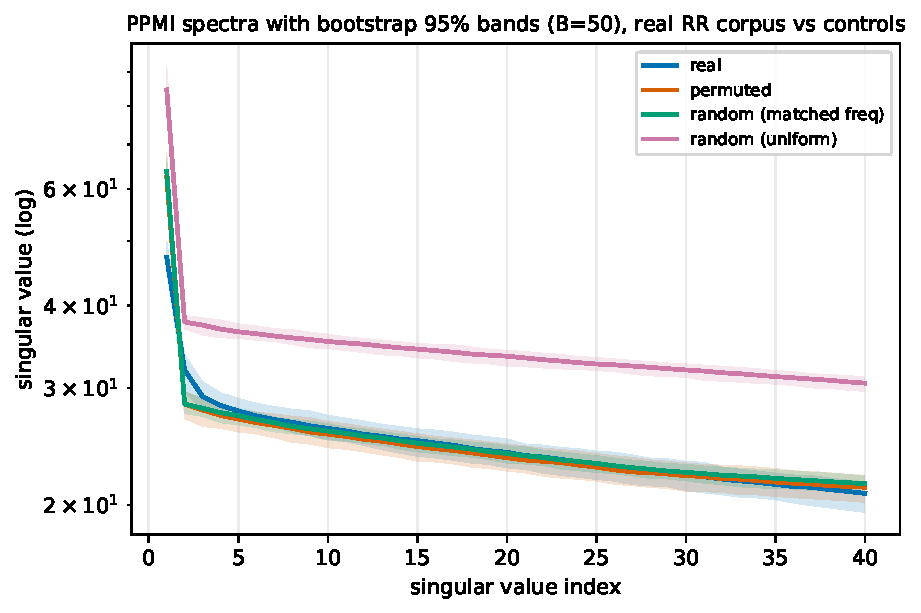
\includegraphics[width=\linewidth]{figures/fig3_spectrum_bootstrap.pdf}
\caption{F3 --- PPMI spectra with bootstrap bands, real RR corpus vs
three controls. \emph{The real spectrum does not separate from the
permuted or frequency-matched controls}: in this short-line regime the
concentration radius of T3 dominates the spectral gap, and no
separation is predicted. Only the uniform control separates
(trivially, by its flat unigram distribution). This is the reported
negative result referenced in \cref{sec:experiments}.}
\label{fig:spectrum-app}
\end{figure}

\begin{figure}[h]
\centering
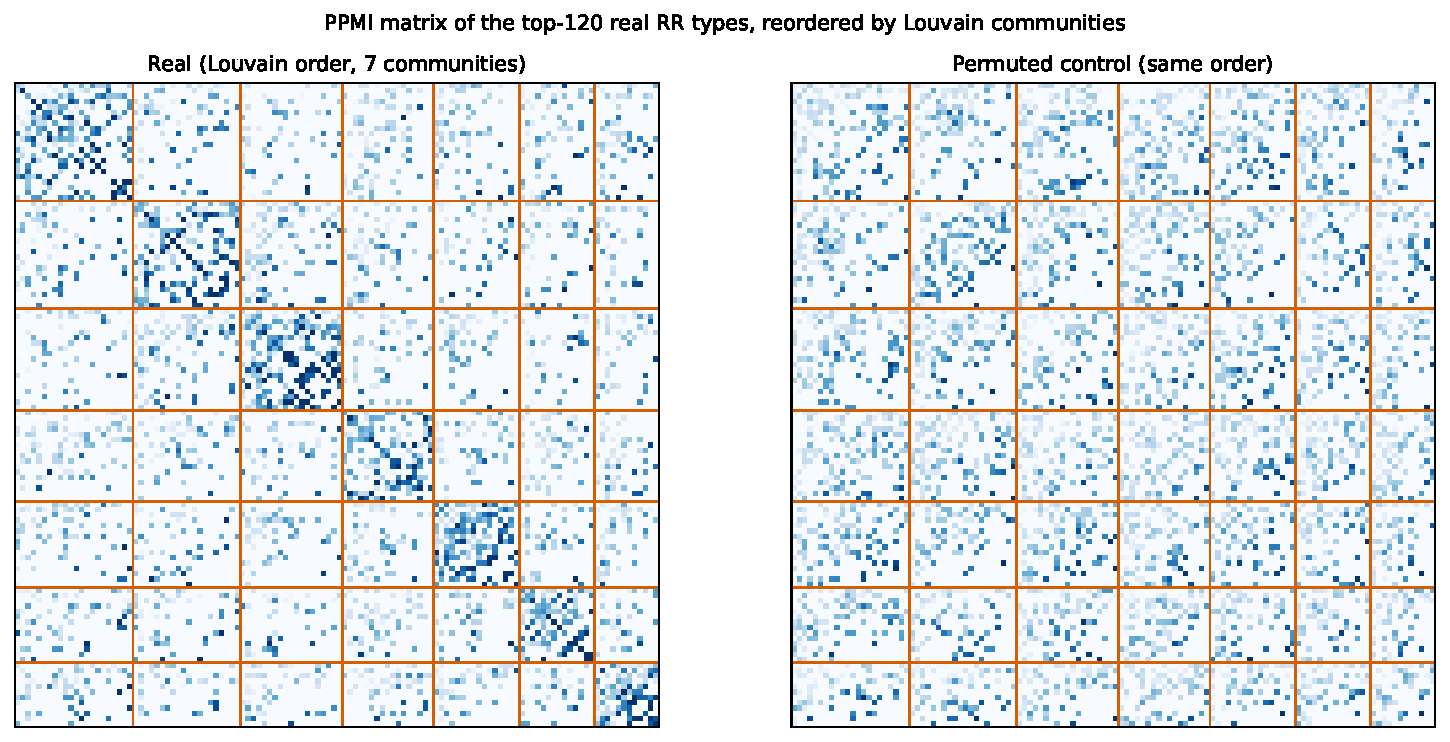
\includegraphics[width=\linewidth]{figures/fig2_ppmi_heatmap.pdf}
\caption{F2 --- PPMI matrix of the top-120 real types reordered by
Louvain communities (7 communities), with the permuted control under
the same ordering. Diagonal blocks evidence co-occurrence communities
(\Cone); \emph{block membership does not identify meaning}.}
\label{fig:heatmap-app}
\end{figure}

\begin{figure}[h]
\centering
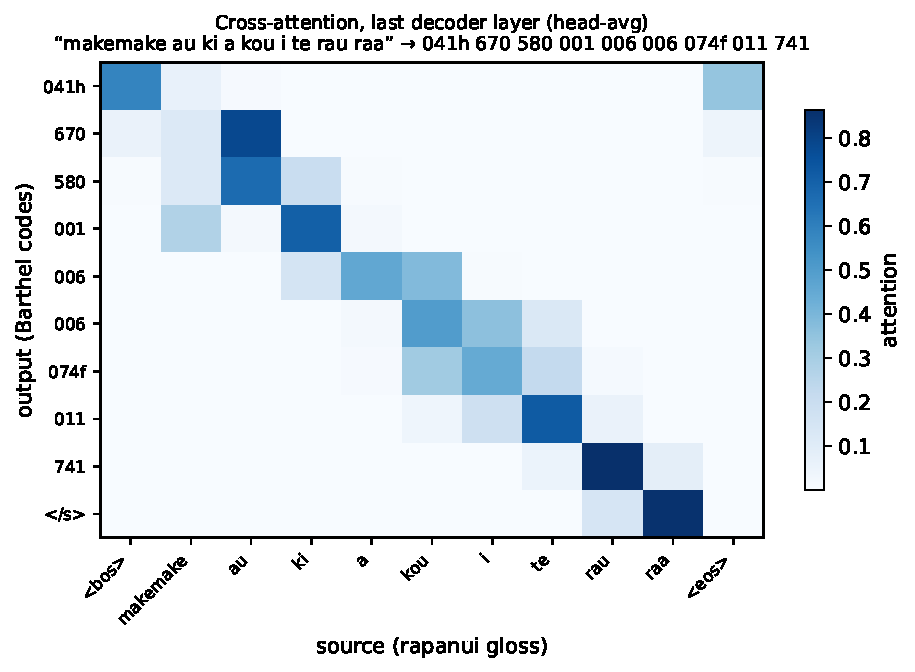
\includegraphics[width=\linewidth]{figures/fig4_attention_map.pdf}
\caption{F4 --- cross-attention (last decoder layer, head-averaged)
for the gloss \emph{makemake au ki a kou i te rau raa}. The formula
\texttt{041h 670 580} attends to the verb \emph{makemake}.
\emph{Attention reflects the learned synthetic mapping; it is not
evidence of any real correspondence.}}
\label{fig:attn-app}
\end{figure}

\begin{figure}[h]
\centering
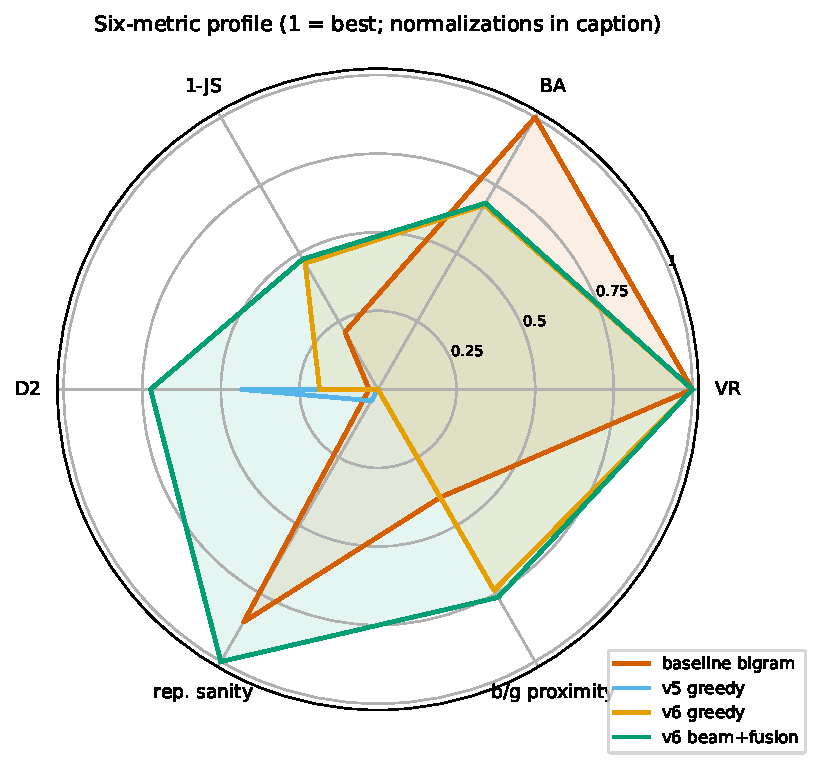
\includegraphics[width=\linewidth]{figures/fig7_radar.pdf}
\caption{F7 --- six-metric profile, normalized to $[0,1]$ (1 = best):
VR, BA, D2 as-is; JS as $1-\mathrm{JS}$; repetition sanity 1 at
RM$\le$2 declining to 0 at RM$\ge$50; b/g as proximity to the real
held-out reference $|b/g-8.26|$ (per P6, raw minimization is not the
target).}
\label{fig:radar-app}
\end{figure}

\begin{figure}[h]
\centering
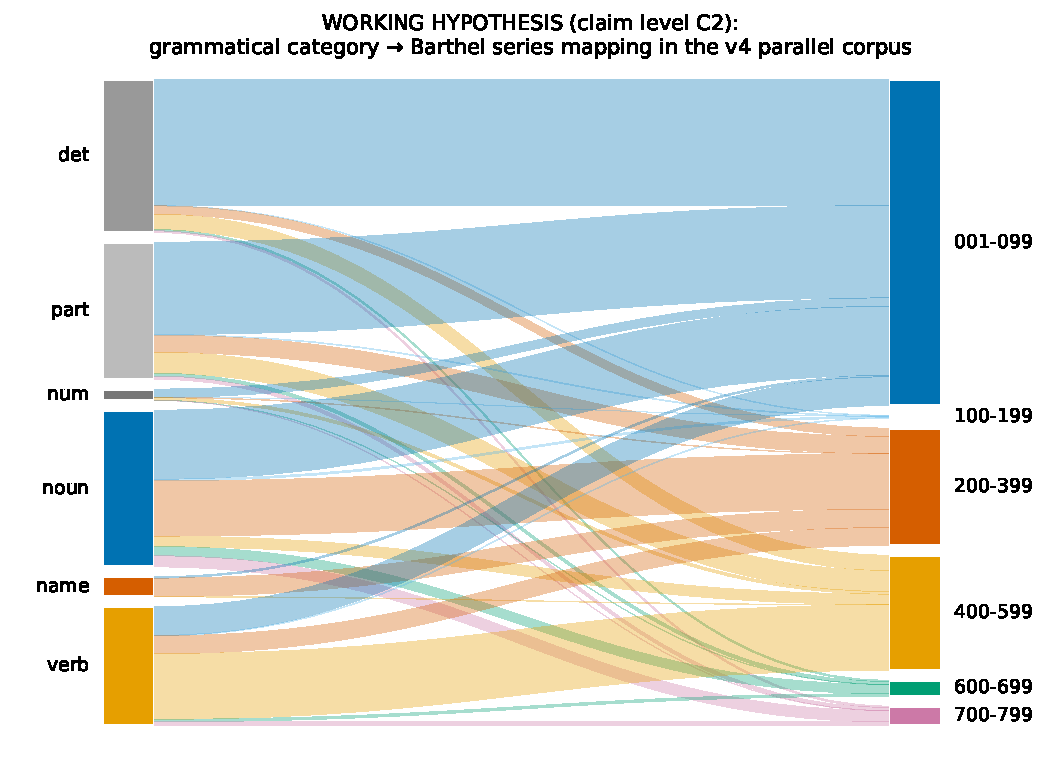
\includegraphics[width=\linewidth]{figures/fig8_sankey_hypothesis.pdf}
\caption{F8 --- the category$\to$Barthel-series mapping of the
parallel corpus, labeled as what it is: a \textbf{working hypothesis
(\Ctwo)}. Flows are counted from the v4 corpus; they encode our
construction, not a discovered correspondence.}
\label{fig:sankey-app}
\end{figure}

\section{Retrained ablations}
\label{app:ablations}

Two ablations require retraining: \emph{no-class-restriction}
(parallel corpus regenerated with every category drawing from the full
Barthel range, seed 42) and \emph{no-augmentation} (masking
augmentation disabled). \textbf{Budget caveat:} both retrained
ablations use an 8-epoch budget (val.\ PPL $14.8$) versus 15 epochs
for the full system (PPL $10.7$); the comparison therefore bounds the
component's contribution at reduced budget rather than at convergence.
Both are decoded with the full beam+fusion configuration.

\begin{table}[h]
\centering
\small
\caption{Retrained ablations (metrics as in Table~1; decoded with
beam-5, $\lambda=0.35$, repetition penalty).}
\begin{tabular}{lccccc}
\toprule
System & BA & JS$\downarrow$ & D2$\uparrow$ & RM & b/g\\
\midrule
full (15 ep.) & 0.68 [.59,.77] & \textbf{0.52} & 0.72 & 2 & 7.31\\
no class restr.\ (8 ep.) & 0.80 [.70,.88] & 0.62 & 0.44 & 2 & 7.02\\
no augmentation (8 ep.) & 0.74 [.65,.83] & 0.48 & 0.77 & 2 & 7.23\\
\bottomrule
\end{tabular}
\end{table}

Removing the class restriction shifts probability mass onto the most
frequent glyphs and transitions: attested-bigram score rises
(0.80 vs.\ 0.68) while unigram-distribution match and diversity
degrade (JS $0.52\to0.62$, D2 $0.72\to0.44$) --- the same trade-off
direction as the count-based baseline, in milder form. This is
evidence that the \Ctwo{} class hypothesis contributes distributional
shape, not just interpretability. Removing augmentation at equal
budget moves all metrics within CI overlap of the full system;
augmentation's measurable contribution at this corpus size is small.

\section{Blind-judge protocol}
\label{app:judges}

Materials (blinded 40-item sheet, sealed key, analysis plan with AUC,
Fleiss $\kappa$, bootstrap CIs) are in
\texttt{reports/blind\_judge\_test/}. The test is pre-registered by
commit hash; results will be reported regardless of outcome.

\end{document}
